% !TeX root=main.tex

\chapter{کارهای مرتبط} \label{ch:related}
\thispagestyle{empty}


\section{مقدمه}
\label{sec:intro}
\paragraph{}
{
    در این فصل به معرفی کارهای مشابه و شرح
    رویکردهای مورد استفاده برای حل مساله‌ی پرسش‌و‌پاسخ تصویری می‌پردازیم.
    در ابتدا به بررسی روش‌های متفاوتی که برای حل مسئله پرسش‌وپاسخ تصویری 
    ارائه شد و سپس به کارهای مشابه با تولید پاسخ در پرسش‌وپاسخ تصویری
    و مجموعه داده‌های موجود در این زمینه پرداخته ‌شده است. در نهایت به 
    مدل‌های از پیش‌ آموزش داده شده در این زمینه می‌پردازیم.  
}

\section{
    روش‌های متفاوت حل مسئله پرسش‌وپاسخ تصویری
}
\label{sec:approches_vqa}
\paragraph{}{
    تا قبل از سال 2019 روش‌ها و رویکرد‌های متفاوتی ارائه شده که 
    بتوان ویژگی‌های تصویری و زبانی را در کنار یکدیگر قرار دهیم. به طور کلی
    این روش‌ها را می‌توان در 5 دسته طبقه بندی کرد. 
}
\subsection{
    روش‌های بر پایه 
    \lr{Bilinear Pooling}    
}
\label{sec:binilear_pooling}
\paragraph{}{
    روشی برای ایجاد توجه بین بردار‌های زبانی و بردار‌های تصویری است. 
    روش‌های 
    \r{Bilinear}
    بازنمایی خوبی را فراهم می‌کردند و در بسیاری از کارهای تصویری استفاده می‌شد. 
    در سال 2016
    روشی با نام 
    \lr{MCB}
    \cite{fukui-etal-2016-multimodal}
    برای ادغام تصویر و زبان ارائه شد. رویکرد آن‌ها در شکل 
    \ref{fig:mcb}
    نشان داده شده‌است. 
    \begin{figure}[H]
        \center{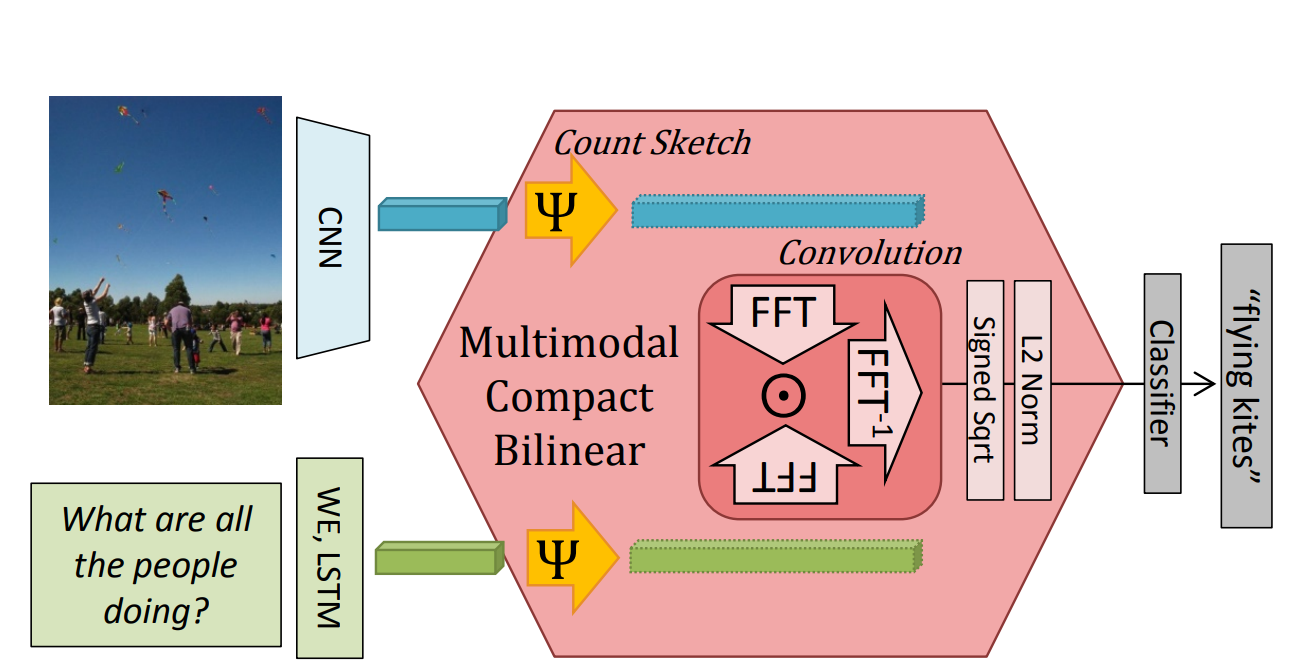
\includegraphics[width=0.7\textwidth]{figs/BiPooling.png}}
        \caption{روش \lr{MCB} برای ادغام تصویر و زبان}
        \label{fig:mcb}
    \end{figure}
    در سال 2017 نیز روشی از 
    دیگر
    با نام 
    \lr{MLB}
    \cite{kim2016hadamard}
    برپایه 
    \lr{Bilinear Pooling}
    را برای مسائل زبان و تصویر منتشر کرد که در زمان خود از 
    مدل‌های پایه‌ای عملکرد بهتری نشان داد. 
}

\subsection{
    روش‌های بر پایه توجه
}
\label{sec:attn_vqa_approach}
\paragraph{}{
    تا قبل از اینکه معماری‌های تبدیل‌کننده معرفی شوند،‌ محققان از مکانیزم توجه
    بر شبکه‌های عصبی بازگشتی و شبکه‌های کانولوشن استفاده می‌کردند، برای مثال
    شبکه‌ توجه پشته‌ای
    \cite{yang2016stacked}
    ،
    توجه سلسه‌مراتبی 
    \cite{NIPS2016_9dcb88e0}
    و 
    توجه متقارن
    \cite{nguyen2018improved}
    پس از ارائه مکانیزم‌های توجه منتشر شدند.
    همان‌طوری که از تصویر 
    \ref{fig:stacked_attention}
    مشخص است، توجه سلسله‌مراتبی 
    برای پردازش تصویر از یک شبکه‌ کانولوشن و برای پردازش سوال یا 
    همان بخش زبانی، از یک 
    \lr{LSTM}
    استفاده شده است، سپس با استفاده از مکانیزم پیشنهادی به تناظر میان این دو بخش
    پرداخته شده است. در هر دو پژوهش مجموعه داده‌های مشهور زبان و تصویر 
    ارزیابی شده‌ و نسبت به مدل‌های 
    \lr{SOTA}
    به خوبی عمل کرده بود. با این‌ حال، این مدل‌ها دارای اشتباهات بسیاری بودند و 
    نیازمند بهبود بودند تا اینکه مدل‌های تبدیل شونده منتشر شدند و 
    توانستند به دقت به نسبت بالاتری از این معماری‌ها برسند.
    \begin{figure}[H]
        \center{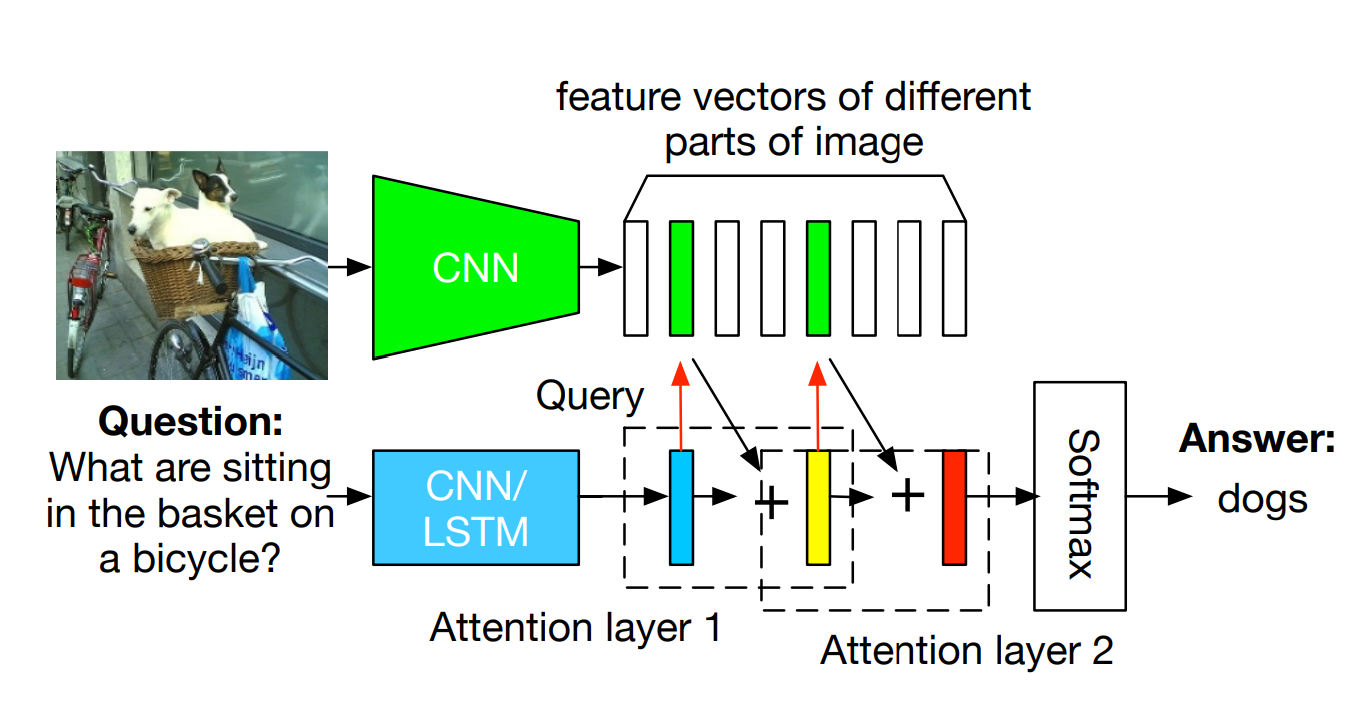
\includegraphics[width=0.7\textwidth]{figs/stacked_attention.png}}
        \caption{توجه پشته‌ای برای حل مسئله پرسش‌وپاسخ تصویری}
        \label{fig:stacked_attention}
    \end{figure}
}

\subsection{
    ادغام روابط اشیاء
}
\label{sec:object_relation_approach}
\paragraph{}{
    یکی از ایده‌های خلاقانه حل مسئله پرسش‌و‌پاسخ تصویری استفاده از شبکه‌های رابطه‌ای
    است که در ابتدا روابط بین اشیاء در تصویر و روابط بین کلمات در سوال مشخص
    می‌شوند و سپس به شبکه‌ای برای پیش‌بینی پاسخ مورد نظر ورودی داده می‌شوند. 
    از نمونه کارآمد این روش می‌توان به مفاله حل پرسش‌وپاسخ تصویری از طریق 
    ساختار گرافی 
    \cite{teney2017graph}
    اشاره کرد که در ابتدا اشیاء موجود در تصویر و روابط بین آن‌ها،‌
    و همچنین کلمات موجود در جمله سوال و روابط بین آن‌ها را
    به صورت گراف توصیف کرده و سپس آن‌ها به شبکه‌ عصبی ورودی می‌دهیم تا 
    بتواند از طریق آن‌ها به پاسخ مورد نظر برسد.
    برای بدست آوردن رابطه بین اشیاء در تصویر می‌توان از شبکه‌های رابطه‌ای 
    و برای بدست آوردن گراف جمله می‌توان از گراف وابستگی گرامری 
    استفاده کرد. 

    \begin{figure}[H]
        \center{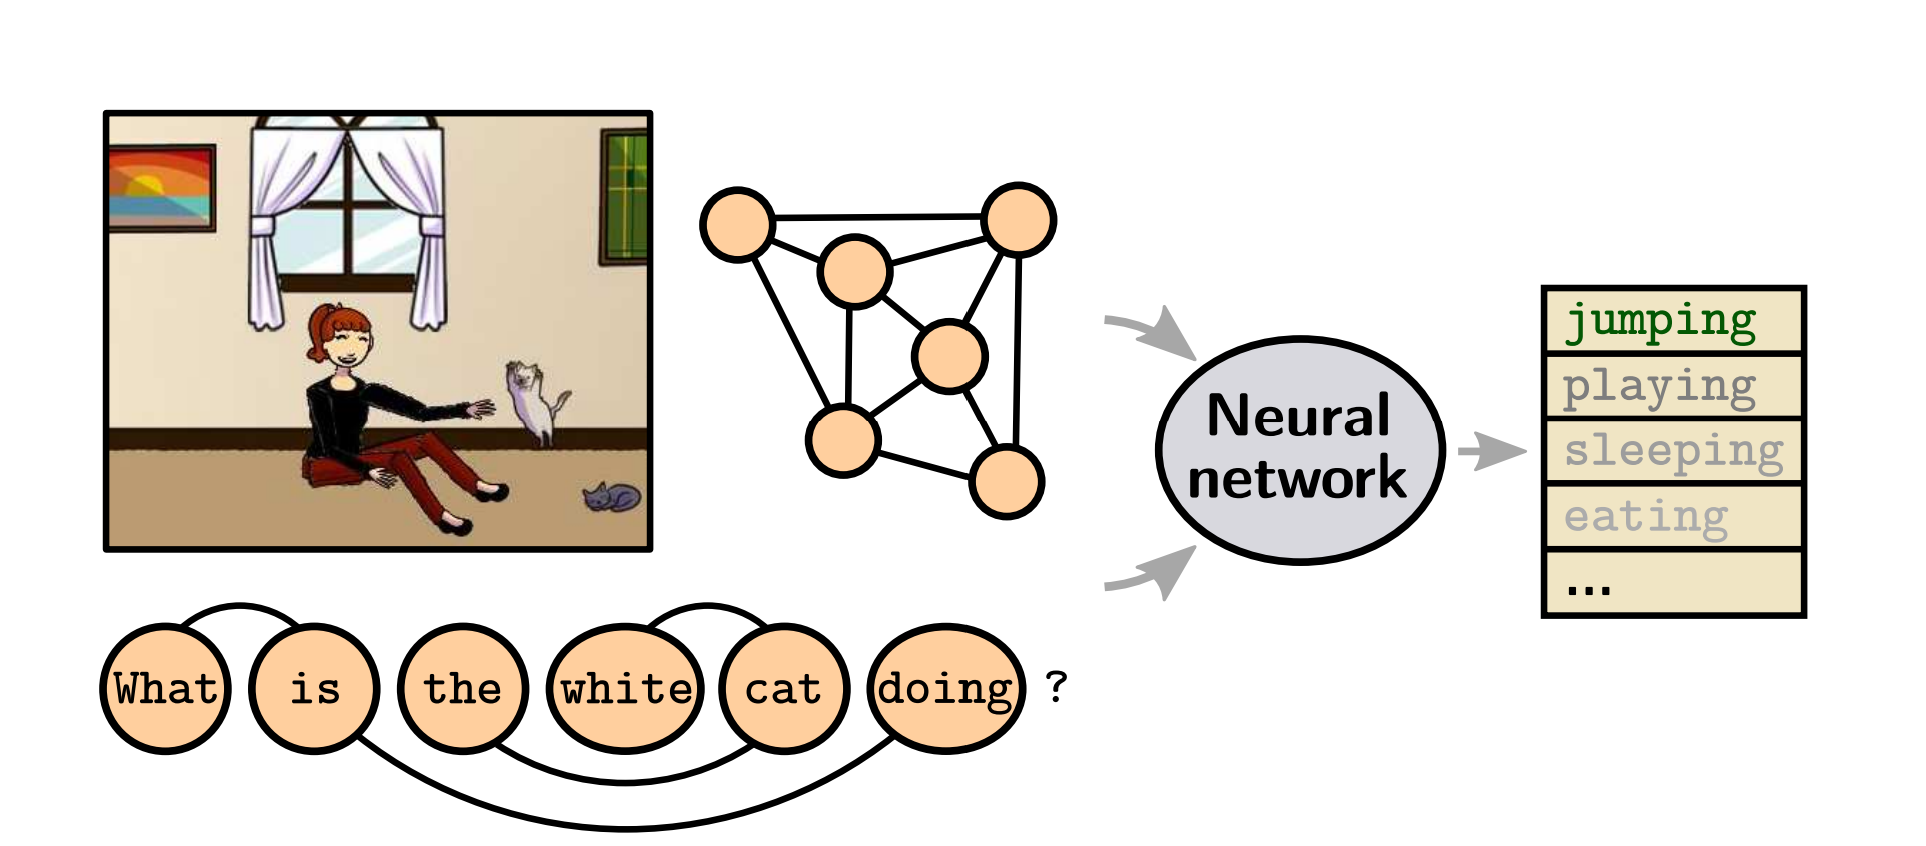
\includegraphics[width=0.7\textwidth]{figs/object_relation.png}}
        \caption{حل پرسش‌وپاسخ تصویری با ساختارهای گرافی}
        \label{fig:object_relation}
    \end{figure}
    
}

\section{
    تولید پاسخ برای پرسش‌و‌پاسخ تصویری
}
\label{sec:answer_generation}
\paragraph{}
{
    همان‌طوری که در بخش 
    \ref{sec:approches_vqa}
    توضیح داده‌شد، تلاش‌های بسیاری برای حل پرسش و پاسخ تصویری از طریق دسته‌بندی
    شده است، در حالی که حل مسئه از طریق تولید متن توجه چندانی از محققان را 
    جلب نکرده‌است. راه‌هایی برای حل پرسش‌وپاسخ تصویری با نام‌های
    \lr{mQA} \cite{gao2015you} 
    و
    \lr{AMA} \cite{wu2016ask} 
    ارائه شد که از شبکه‌های 
    \lr{LSTM} 
    برای تولید پاسخ استفاده شده بود. 
    پس از آن نیز سیستم‌هایی نظیر 
    \lr{SimVLM} \cite{wang2021simvlm}
    منتشر شد که هدف آن کاهش هزینه و پیچیدگی آموزش بود. در این 
    سیستم‌ها حل کردن مسائل مرتبط با زبان و تصویر به هر دو روش
    تولید پاسخ و دسته‌بندی بررسی شده است. 
    در نهایت، 
    \lr{VL-Bart} و \lr{VL-T5} \cite{pmlr-v139-cho21a}
    یک چهارچوب یکپارچه‌ای را ارائه کردند که توانایی آموزش 
    کار‌های متفاوتی در کنار یکدیگر را داشت. شکل
    \ref{fig:vl-bart}
    کارایی این چهارچوب را در بخش های مختلف نشان می دهد.
    این مدل‌ها نشان‌ دادند که
    حل کردن مسائل چند ماژول از طریق تولید متن عملکرد و کارایی بهینه‌تری 
    از دسته‌بندی دارد. با این حال، از آنجایی که 
    این مدل‌ها روی مجموعه داده پرسش‌وپاسخ تصویری 
    \cite{VQA}
    آموزش داده شده‌اند و پاسخ‌ها در این مجموعه داده به صورت دسته‌بندی داده
    شده است، همچنان پاسخ دادن به صورت جملات را در بر ندارند.
    \begin{figure}[H]
        \center{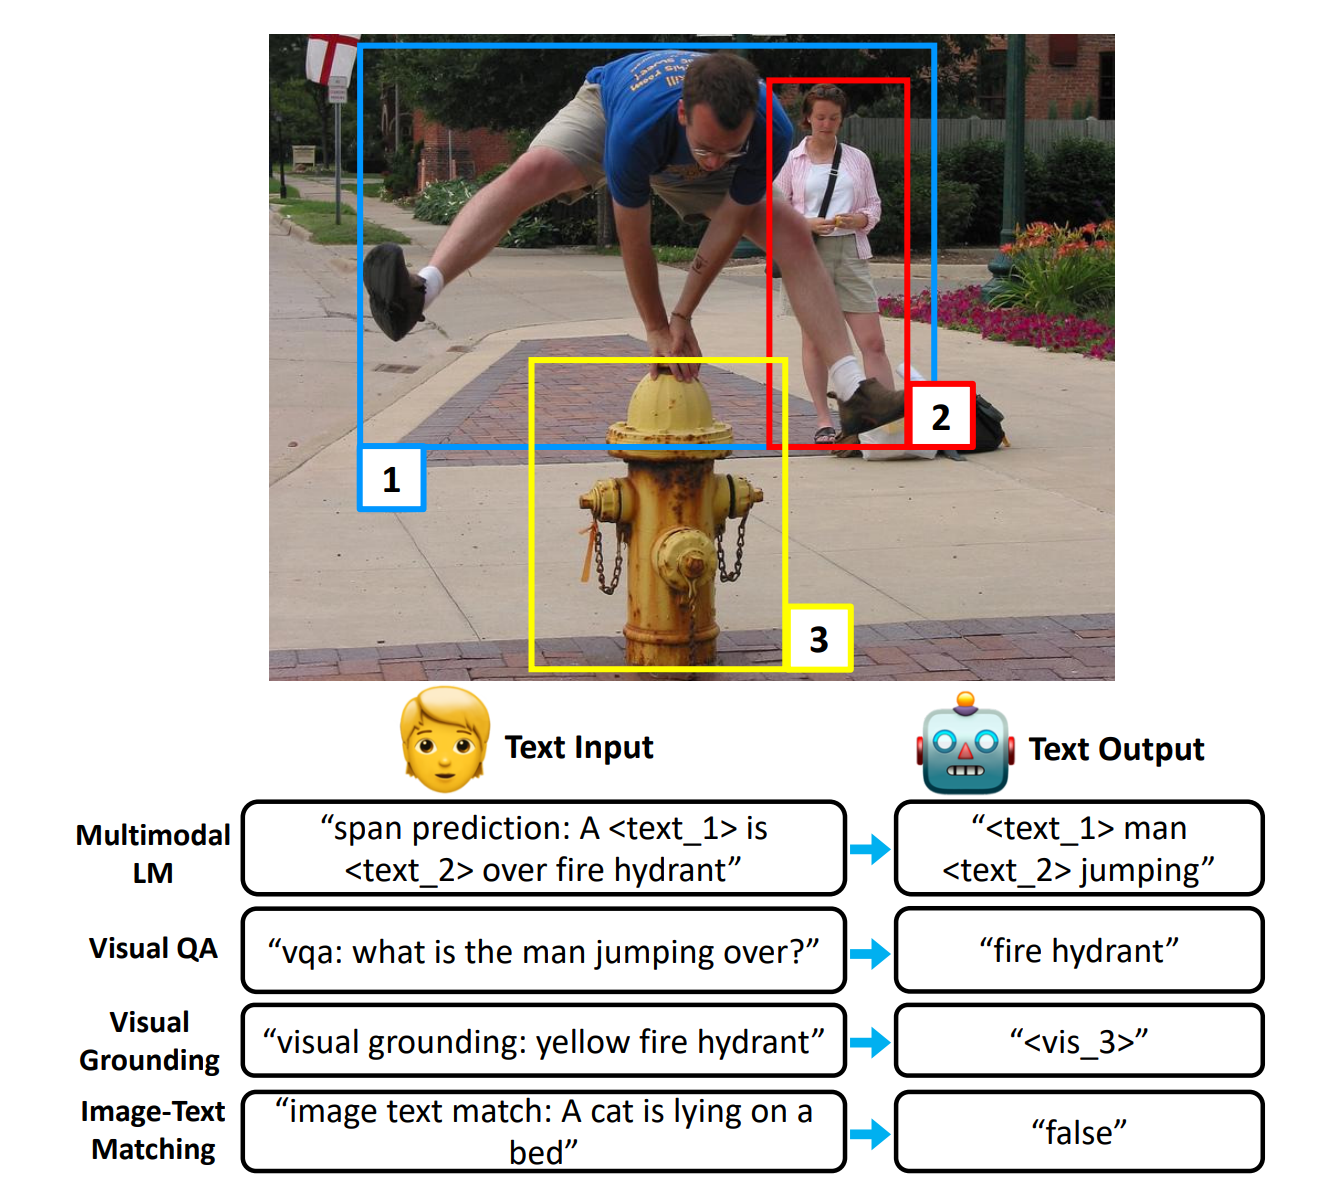
\includegraphics[width=0.7\textwidth]{figs/VL-BART.png}}
        \caption{چهارچوب یکپارچه ارائه شده برای حل مسائل چند ماژول به روش تولید متن}
        \label{fig:vl-bart}
    \end{figure}

}

\section{مجموعه داده‌های منتشر شده در پرسش‌وپاسخ تصویری}
\label{sec:vqa_datasets}
\paragraph{}
{
    مجموعه داده‌های زیادی در حوزه پرسش‌وپاسخ تصویری ارائه شده است. 
    با این حال، بسیاری از مجموعه داده‌ها دارای پاسخ‌های تک‌کلمه‌ای هستند 
    و تعداد کمی از آن‌ها پاسخ‌ها را به صورت جمله نوشته‌اند. 
    در سال 2019 مقاله 
    \lr{VCR} \cite{zellers2019recognition}
    ارائه شد که یک سوال چالشی از تصویری پرسیده شود و در جواب آن باید 
    پاسخی همراه با دلیل انتخاب پاسخ خروجی داده شود. 
    این مجموعه داده شامل 
    290 هزار 
    پرسش و پاسخ چند گزینه‌ای است که از 110 هزار صحنه فیلم‌ها گرفته شده است. 
    این مجموعه داده نشان داد که بر خلاف ساده بودن 
    \lr{VCR}
    برای انسان‌ها
    (دقتی بالاتر از 90)
    ماشین‌ها توانایی چندانی در حل آن ندارند. نویسندگان، مدلی نیز ارائه دادند که این
    مسئله را حل کند، ولی  طبق ادعای آن‌ها این مسئه همچنان فاصله زیادی تا حل دارد. 
    
    \begin{figure}[H]
        \center{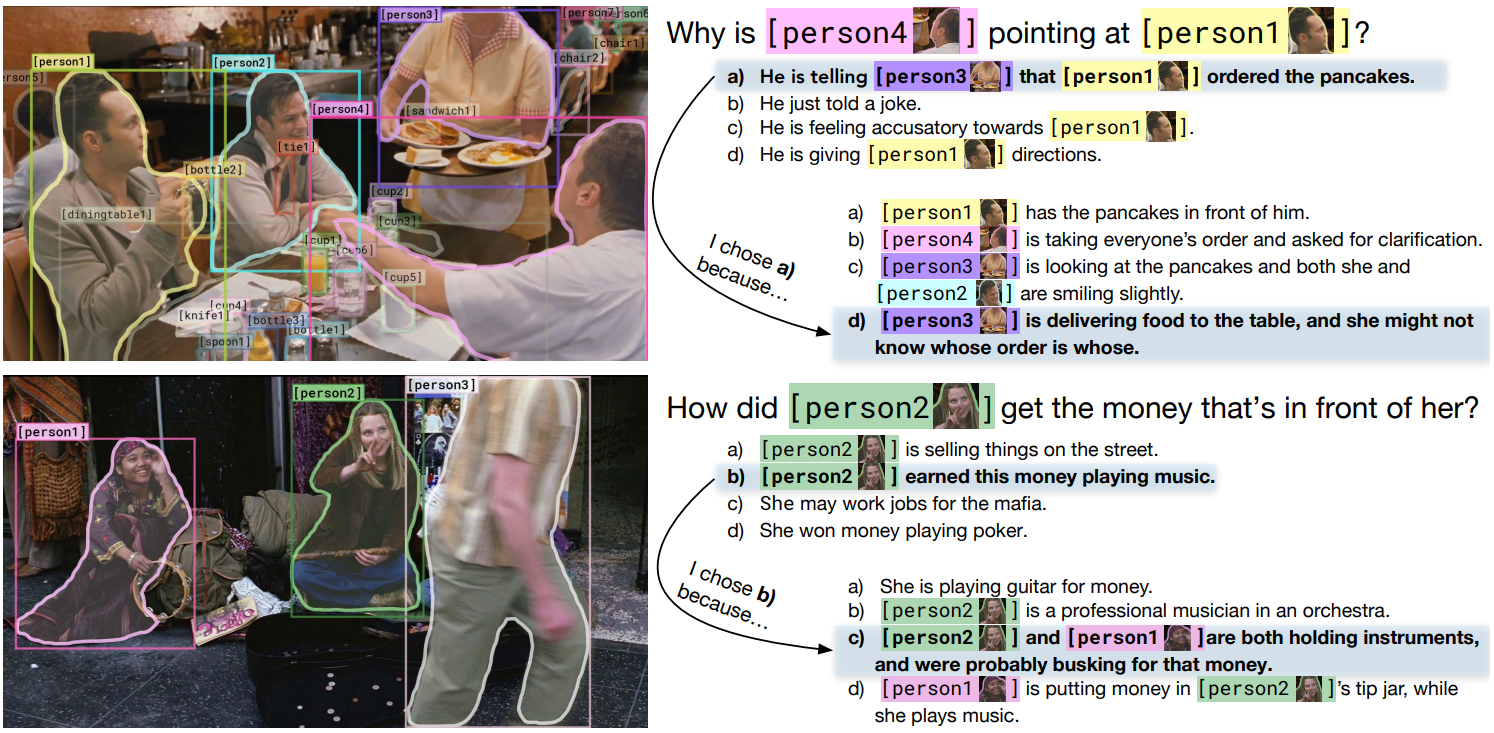
\includegraphics[width=1\textwidth]{figs/VCR.png}}
        \caption{نمونه‌ای مجموعه داده 
        \lr{VCR}
        که علاوه بر ارائه پاسخ، نیازمند ارائه دلیلی برای پاسخ است}
        \label{fig:vcr}
    \end{figure}
    مجموعه داده‌ دیگری با نام 
    \lr{VQA-E} \cite{li2018vqa}
    منتشر شد که برگرفته در مجموعه داده رسمی پرسش‌وپاسخ تصویری بود. 
    برای حل این مجموعه داده، علاوه بر ارائه پاسخ 
    (تک‌کلمه‌ای)
    باید توضیحی برای پاسخ انتخاب شده ارائه شود. نحوه تولید این مجموعه داده
    به این صورت است که به ازای هر سه‌تایی پرسش، تصویر و پاسخ یک توضیحی 
    با توجه به توضیحات تصویر تولید می‌شود. در این مجموعه داده، تلاش بر این بوده
    که توزیعی مشابه با مجموعه داده رسمی پرسش‌وپاسخ تصویری داشته باشد. 
    مجموعه داده‌های دیگری نیز به صورت جمعیت‌‌محور ارائه شده‌اند. این مدل مجموعه
    داده‌ها می‌توان به 
    \lr{A-OKVQA} \cite{schwenk2022okvqa}
    اشاره کرد که شامل 25 هزار پرسش است. 
}

\section{ مدل‌های از پیش آموزش‌ داده‌شده}
\label{sec:vlp}
\paragraph{}
{
    پیش‌آموزش مدل‌های زبان-تصویر اخیرا مورد توجه بسیاری واقع شده است. مدل‌های 
    موجود بیش‌تر بر پایه توجه به خود و معماری تبدیل شونده که در بخش ‌های
    \ref{subsec:self_attn}
    و
    \ref{sec:transformers}
    به صورت جزئی مورد بررسی قرار گرفته‌اند. این مدل‌ها در هر دو بخش 
    تصویر و زبان به خوبی عمل کرده‌اند. 
    همانطوری که در بخش
    \ref{sec:bertlike_arcs}
    توضیح داده‌شد، این مدل‌ها را می‌توان به دو بخش تک‌جریان و دو جریان دسته‌بندی 
    کرد. 
    با توجه به اینکه این مدل‌ها در تولید متن استفاده چندانی نداشته‌اند، در این
    پژوهش تلاش بر این بوده که مدل‌های از‌ پیش آموزش داده‌شده را برای این هدف 
    استفاده کنیم. 
}